\chapter{Introduction}
\label{chap:introduction}



\section{Novozymes and biotechnology}


Novozymes A/S (\ac{NZ}) is a company whose line of business consists of the development of products performing chemical transformations in economically relevant processes. The application of these products, instead of conventional solutions, has the advantage of requiring less chemical substances, potentially simplifying industrial processes, reducing their costs and their environmental impact \cite{madigan2000brock}. Notorious examples of such applications include waste-water treatment, household care or fermentation. For example, a product called Fermax was recently released to prevent foam development during the sugarcane ethanol production (see figure \ref{fig:ethanol}).

\begin{figure}[!h]
\centering
  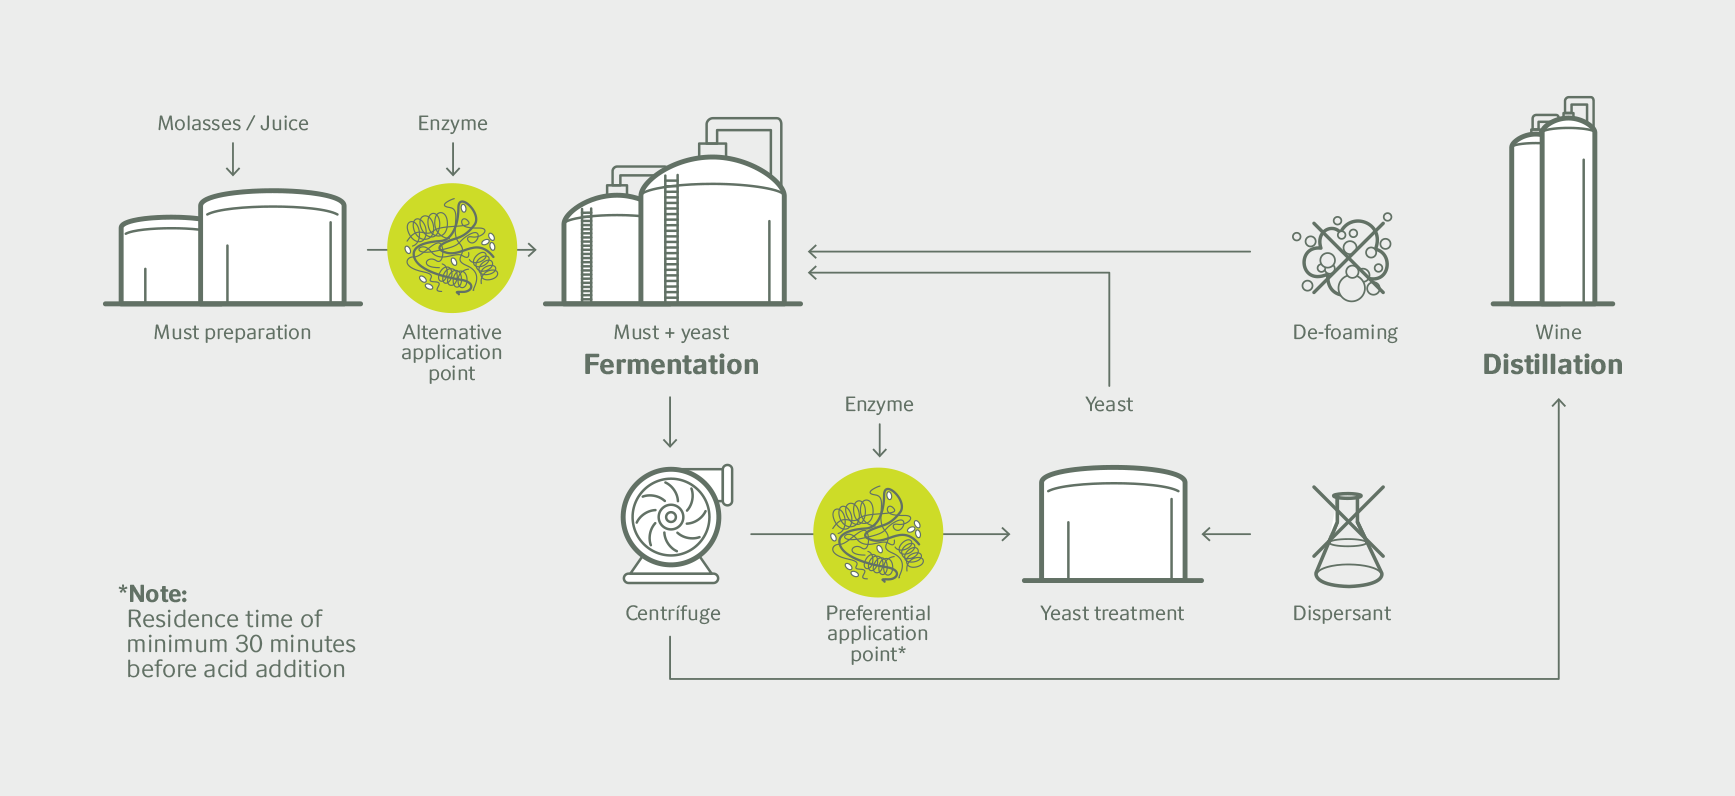
\includegraphics[width=\textwidth]{fermax}
\caption[Example of bioprocess optimised by Novozymes]{Schematic representation of a bioindustrial process optimised with a Novozymes product, marked as a green circle. Taken from Novozymes intranet.}
\label{fig:ethanol}
\end{figure}

The company\textquotesingle s name is inspired by the molecular agents that power these transformations, \textbf{enzymes}. Enzymes consist of an extremely diverse family of molecules catalyzing a plethora of biochemical reactions happening in living beings, from bacteria to humans \cite{Nelson2008}. 

\ac{NZ} takes advantage of these molecules by matching processes where a chemical transformation takes place, with an enzyme that could improve its efficiency, defined in terms of resource consumption, speed or waste subproduction. Moreover, \ac{NZ} thrives to improve the performance of the selected enzymes in the target process by modifying its Wild Type (WT) form. Proteomics plays a key role on the research process required, thus \ac{NZ} has a keen interested in being at the vanguard of research and tool development in this field.

\section{Bioinformatics and proteomics}

The majority of enzymes consist of proteins. But what are proteins? Proteins are molecules made up of 20 basic units, called aminoacids. All aminoacids share a common chemical structure, where a carbon atom ($C_\alpha$) is covalently bonded to a hydrogen atom, a carboxyl group (\ce{-COOH}), an amino group (\ce{-NH_2}), and last but not least, a radical, also called side chain of the aminoacid. A slight deviation from this pattern exists in proline, where the radical is bound to the nitrogen atom, making it an iminoacid. The side chain differs between aminaocids and creates the aminoacidic diversity   (see figure \ref{fig:aminoacids}).

\begin{figure}
  \centering
  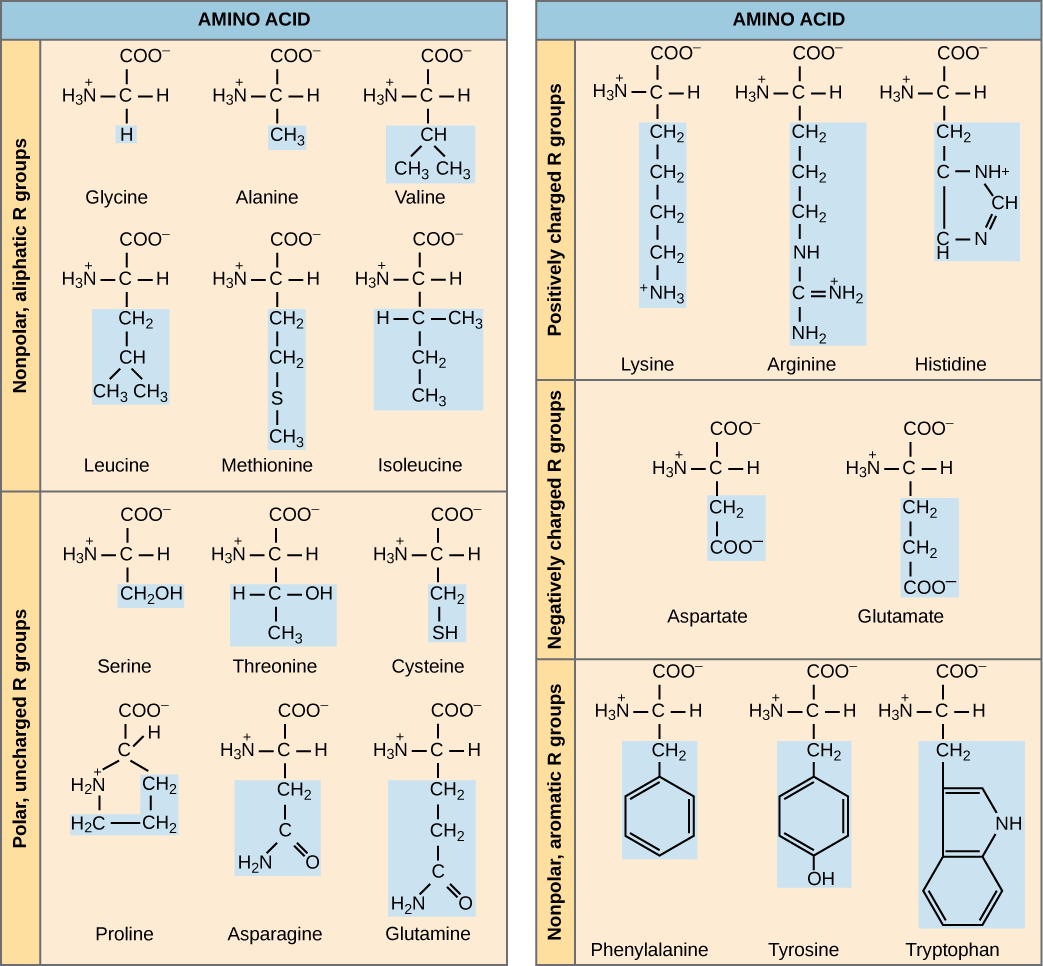
\includegraphics[width=0.8\textwidth]{aminoacids2.png}
  \caption[The 20 aminoacids]{Molecular structure of the 20 aminoacids, organized by chemical properties into five groups. Taken from \href{https://cnx.org/contents/vxf032Bc@4/Proteins}{https://cnx.org/contents/vxf032Bc@4/Proteins}.}
  \label{fig:aminoacids}
\end{figure}

The carboxyl group and amino group of different aminoacids can undergo a dehydration that generates a covalent bond, called peptidic bond, subsequently joining two aminoacids (see figure \ref{fig:peptidic_bond}). The remaining amino and carboxyl groups can in turn be joined to new aminoacids, giving way for the formation of a biopolymer, where each subunit is an aminoacid. A peptide consists of a small chain of aminoacids joined this way. If made long enough, it acquires complex structures and becomes a protein \cite{Nelson2008}.

\begin{figure}
  \centering
  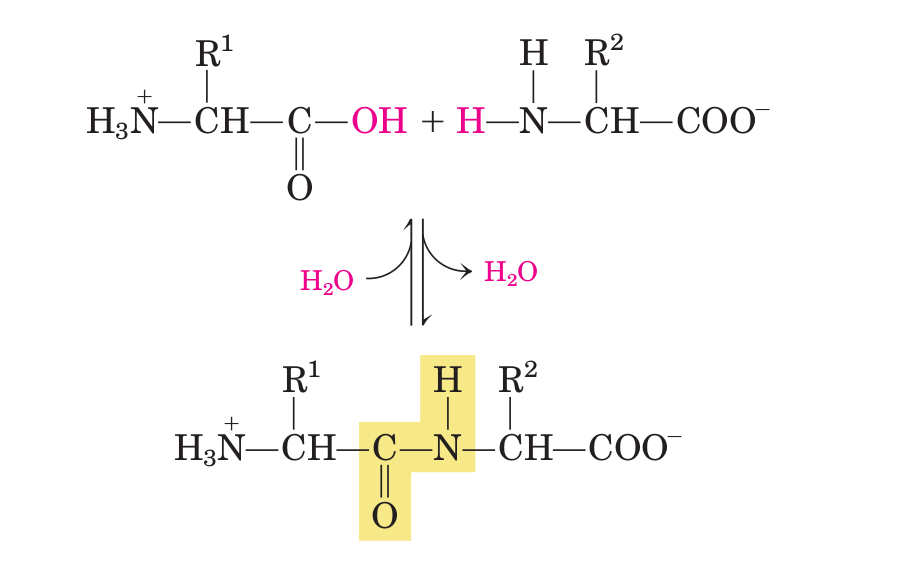
\includegraphics[width=0.8\textwidth]{peptidic_bond.png}
  \caption[The peptidic bond]{The peptidic bond brings together different aminoacids into a single protein. Taken from \cite{Nelson2008}.}
  \label{fig:peptidic_bond}
\end{figure}


Proteomics is the branch of bioinformatics whose purpose is the application of algorithms and data analysis to biological studies dealing with proteins. With proteomics, one endeavors to infer the protein composition of a sample, and subsequently quantify its protein abundances. 

More concretely, proteomics studies how proteins are capable of coordinating their functions by means of complex systems of regulation.  Proteomics aims at unraveling this complexity, and understanding how its powerful properties emerge from its individual components \cite{Milo2002}. For instance, the interplay of proteomics and biotechnology helps researchers learn which proteins are key in the onset of disturbances to these regulations \cite{Saraon2012}. The application of proteomics to biological problems is not restricted to medical problems such as cancer, but also biotechnological processes like those carried out by \ac{NZ}.





\section{Objectives of the Thesis}
\label{sec:objectives}

In line with the goal of advancing \ac{NZ} capabilities in proteomics research, with the final ambition of speeding the research turnover in the company, this project aimed at the following:

\begin{enumerate}

\item Develop an open-source, Linux based and easily deployable pipeline for the analysis of proteomics data, starting at the raw high-throughput data files and ending in the  biological interpretation of the results.

\item Propose a label-free quantification probabilistic model that provides relative abundance estimates and a measurement of their uncertainty based on the available data.


\item Evaluate the tools with benchmark datasets to assess their performance and check they convey the biological phenomena captured in the data.



\end{enumerate}

\section{Structure of the Thesis}

An overview over the main data collection technique used in proteomics, Mass Spectrometry (\ac{MS}), and the ensuing computational data analysis steps is presented in chapter \ref{chap:mass_spec}. An inspection of the developed pipeline is provided in chapter \ref{chap:pipeline}, while the probabilistic model is introduced in chapter \ref{chap:model}. A benchmark of both tools on a \ac{NZ} dataset is given in chapter \ref{chap:benchmark}. Finally, a conclusion of the work is given in chapter \ref{chap:conclusion}.
